\documentclass[
	% -- opções da classe memoir --
	12pt,				% tamanho da fonte
	openright,			% capítulos começam em pág ímpar (insere página vazia caso preciso)\
	oneside,			% para impressão em verso e anverso
	a4paper,			% tamanho do papel. 
	% -- opções da classe abntex2 --
	chapter=TITLE,		% títulos de capítulos convertidos em letras maiúsculas
	% -- opções do pacote babel --
	english,			% idioma adicional para hifenização
	brazil				% o último idioma é o principal do documento
]{ifsc-tcc-abntex2}

%---------------------------------------------------------------------%
%---------------------------------------------------------------------%
% Informações de dados para CAPA e FOLHA DE ROSTO
%---------------------------------------------------------------------%
%---------------------------------------------------------------------%

\titulo{Título da Monografia}
\autor{Nome do Autor}
\local{Florianópolis}
\data{2021}
\orientador[Orientador:\\]{}
\coorientador[Coorientador:\\]{}
\tipotrabalho{Monografia (Graduação)}

% O preambulo deve conter o tipo do trabalho, o objetivo, o nome da instituição e a área de concentração 
\preambulo{Trabalho de conclusão de curso submetido ao Instituto Federal de Educação, Ciência e Tecnologia de Santa Catarina como parte dos requisitos para obtenção do título de engenheiro eletrônico}

\textoaprovacao{Este Trabalho foi julgado adequado para obtenção do Título de Engenheiro Eletrônico em março de 2021 e aprovado na sua forma final pela banca examinadora do Curso de Engenharia Eletrônica do instituto Federal de Educação Ciência, e Tecnologia de Santa Catarina.}


%---------------------------------------------------------------------%
% Início do documento
%---------------------------------------------------------------------%

\begin{document}

\selectlanguage{brazil}
\frenchspacing


% ----------------------------------------------------------
% ELEMENTOS PRÉ-TEXTUAIS
% ----------------------------------------------------------
\pretextual

\imprimircapa
\imprimirfolhaderosto* %(o * indica que haverá a ficha bibliográfica)

%---------------------------------------------------------------------%
% ATENÇÃO - Pergunte para a Biblioteca do IFSC
% Inserir a ficha bibliografica - 
%
% Para gerar a ficha catalográfica acesse:
% http://ficha.florianopolis.ifsc.edu.br/
% Precisa ser feito pelo navegador Mozilla Firefox
%---------------------------------------------------------------------%

%\imprimirficha{pdf/fichacatalografica.pdf}
\cleardoublepage

%---------------------------------------------------------------------%
% Inserir folha de aprovação
%---------------------------------------------------------------------%

\imprimiraprovacao
\cleardoublepage

%---------------------------------------------------------------------%
% Dedicatória
%---------------------------------------------------------------------%
\imprimirdedicatoria{Este trabalho é dedicado às crianças adultas que,\\quando pequenas, sonharam em se tornar cientistas.}
% ---

%---------------------------------------------------------------------%
% Agradecimentos
%---------------------------------------------------------------------%
\begin{agradecimentos}
	
	< Texto de Agradecimentos >
	
	%\marcador{add}{Tanta gente...}
\end{agradecimentos}
% ---

%---------------------------------------------------------------------%
% Epígrafe
%---------------------------------------------------------------------%
\begin{epigrafe}
	\vspace*{\fill}
	\begin{flushright}
		\textit{``Uma Epigrafe\\
			uma inspiração.'' \\
			(Autor desconhecido)}
	\end{flushright}
\end{epigrafe}


%---------------------------------------------------------------------%
% RESUMOS
%---------------------------------------------------------------------%
\setlength{\absparsep}{18pt} % ajusta o espaçamento dos parágrafos do resumo
\begin{resumo}
	
	No resumo deve-se ressaltar de forma clara e sintética a natureza e o objetivo do trabalho, o método que foi empregado, os resultados e as conclusões mais importantes, seu valor e originalidade. O resumo é a “apresentação concisa dos pontos relevantes de um texto. Constitui elemento essencial em textos de natureza técnico-científica” (ASSOCIAÇÃO BRASILEIRA DE NORMAS TÉCNICAS, 2003, p.3). O resumo não pode	ultrapassar 250 palavras. Abaixo do resumo devem aparecer as palavras-chave (mínimo três, máximo cinco, separadas por ponto final e iniciadas com letra maiúscula).
	
	\textbf{Palavras-chave}: mínimo três. máximo cinco. separadas por ponto final e iniciadas com letra maiúscula.
\end{resumo}
\begin{resumo}[Abstract]
	\begin{otherlanguage*}{english}
		
		É obrigatório que se faça o resumo na língua vernácula e em língua estrangeira (inglês) – neste último caso, é o chamado abstract. Abaixo do
		abstract devem aparecer as keywords (palavras-chave), em no mínimo três e no máximo cinco, separadas por ponto final e iniciadas com letra maiúscula.
				
		\vspace{\onelineskip}
		
		\noindent 
		\textbf{Keywords}: Keyword. Keyword. Keyword. Keyword. Keyword.
	\end{otherlanguage*}
\end{resumo}


%---------------------------------------------------------------------%
% inserir lista de ilustrações
%
% Nota: Somente deve aparecer em trabalhos com número de ilustrações  (desenhos,  esquemas,  fluxogramas,  fotografias,  gráficos,  mapas, plantas ou quadros) igual ou superior a cinco. Quando esse número for inferior a cinco, a lista de ilustrações é opcional. 
%---------------------------------------------------------------------%
\pdfbookmark[0]{\listfigurename}{lof}
\listoffigures*
\cleardoublepage

%---------------------------------------------------------------------%
% inserir lista de tabelas
%
% Nota:  Somente deve aparecer em trabalhos com cinco ou mais tabelas (quando inferior a cinco é opcional). 
%---------------------------------------------------------------------%
\pdfbookmark[0]{\listtablename}{lot}
\listoftables*
\cleardoublepage

%---------------------------------------------------------------------%
% inserir lista de códigos fonte (listings)
%---------------------------------------------------------------------%
\pdfbookmark[0]{\lstlistlistingname}{lol}
\listoflistings
\cleardoublepage

%---------------------------------------------------------------------%
% inserir lista de abreviaturas e simbolos
%
% Nota: Consiste  na  relação  alfabética  das abreviaturas e siglas utilizadas no texto, seguidas das palavras ou expressões correspondentes grafadas por extenso. Somente deve aparecer no trabalho se tiver um número de siglas igual ou superior a cinco (quando inferior a cinco é opcional).
% Obs: Se não houver nenhuma abreviatura ou símbolos sendo utilizados, haverá um erro ao tentar executar os dois comandos abaixo.
%---------------------------------------------------------------------%
\imprimirlistadeabreviaturas
\imprimirlistadesimbolos
\cleardoublepage
%\usepackage{Simbolos}

%---------------------------------------------------------------------%
% inserir o sumario
%---------------------------------------------------------------------%
\pdfbookmark[0]{\contentsname}{toc}
\tableofcontents*
\cleardoublepage

% ----------------------------------------------------------
% ELEMENTOS TEXTUAIS
% ----------------------------------------------------------
\textual

% Cria a lista de Símbolos/Unidades, Abreviaturas/Siglas, visível somente com \imprimirlistadeabreviaturas e \imprimirlistadesimbolos
% --- Lista de símbolos ---

\simbolo{\si{\watt}}{watt - Unidade de potência elétrica}
\simbolo{\si{\volt}}{volt - Unidade de potencial elétrico}
\simbolo{\si{\second}}{segundos - Unidade de tempo}
\simbolo{\si{\henry}}{henry - Unidade de indutância}
\simbolo{\si{\ampere}}{ampère - Unidade de corrente elétrica}
\simbolo{\si{\hertz}}{hertz - Unidade de frequência}
\simbolo{\si{\farad}}{farad - Unidade de capacitância}
\simbolo{\si{\ohm}}{ohm - Unidade de resistência elétrica}
\simbolo{\si{\coulomb}}{coulomb - Unidade de carga elétrica}

\begin{siglas}
	\item[SMPS] \textit{Switched Mode Power Supply} - Fonte chaveada
	\item[CC] Corrente Contínua
	\item[CA] Corrente Alternada
	\item[EMC] \textit{Electromagnetic Compatibility} - Compatibilidade Eletromagnética
	\item[EMI] \textit{Electromagnetic Interference} - Interferência Eletromagnética
	\item[EMS] \textit{Electromagnetic Suscptibility} - Susceptibilidade Eletromagnética
	\item[CISPR] \textit{Comité International Special des Perturbations Radioélectriques} - Comitê Especial Internacional de Rádio Interferência
	\item[ESD] \textit{Electrostatic Discharge} - Descarga Eletrostática
	
	\item[PCI] Placa de Circuito Impresso
	
	\item[EMP] \textit{Electromagnetic Pulse} - Pulso Eletromagnético
	\item[FCC] \textit{Federal Communication Commission}
	
	\item[IEC] \textit{International Electrotechnical Commission}
	\item[LISN] \textit{Line Impedance Stabilization Network}
	\item[NFP] \textit{Near-Field Probe} - Sonda de Campo Próximo
	\item[DUT] \textit{Device Under Test} - Dispositivo Sob Teste
	\item[OATS] \textit{Open-Area Test Site} - Local de Teste de Área Aberta
	\item[SAC] \textit{Semi Anechoic Chamber} - Câmara Semi Anecoíca
	\item[CI] Circuito Integrado
	\item[IFSC] Instituto Federal de Educação Ciência e Tecnologia de Santa Catarina
	\item[VDC] \textit{Voltage Direct Current} - Tensão Contínua
	\item[VAC] \textit{Voltage Alternating Current} - Tensão Alternada
	\item[ABNT] Associação Brasileira de Normas Técnicas
	\item[abnTex] Normas para \LaTeX
	\item[PTH] Through-Hole Technology
	\item[SMD] Surface-Mount Device
	\item[ESR] Equivalent Series Resistance
\end{siglas}

%%%%%%%%%%%%%% Como usar o pacote acronym
% \ac{acronimo} -- Na primeira vez que for citado o acronimo, o nome completo irá aparecer seguido do acronimo entre parênteses. Na proxima vez somente o acronimo irá aparecer. Se usou a opção footnote no pacote, entao o nome por extenso irá aparecer aparecer no rodapé
%
% \acf{acronimo} -- Para aparecer com nome completo + acronimo
% \acs{acronimo} -- Para aparecer somente o acronimo
% \acl{acronimo} -- Nome por extenso somente, sem o acronimo
% \acp{acronimo} -- igual o \ac mas deixando no plural com S (ingles)
% \acfp{acronimo}--
% \acsp{acronimo}--
% \aclp{acronimo}--
%\begin{acronym}
%	\acro{ABNT}{Associação Brasileira de Normas Técnicas}
%	\acro{abnTeX}{ABsurdas Normas para TeX}
%	\acro{AC}{Autoridade Certificadora}
%	\acro{AES}{\textit{Advanced Encryption Standard}}
%	\acro{TLS}{\textit{Transport Layer Security}}
%	\acro{TPC}{Terceira Parte Confiável}
%\end{acronym}

% ----------------------------------------------------------
% Inclusão dos capítulos que estão em outros arquivos .tex
% ----------------------------------------------------------
%%%%%%%%%%%%%%%%%%%%%%%%%%%%%%%%%%%%%%%%%%%%%%%%%%%%%%%%%%%%%%%%%%%
%%%%%%%%%%%%%%%%%%%%%%%%%%%%%%%%%%%%%%%%%%%%%%%%%%%%%%%%%%%%%%%%%%%
\chapter{Introdução}
%%%%%%%%%%%%%%%%%%%%%%%%%%%%%%%%%%%%%%%%%%%%%%%%%%%%%%%%%%%%%%%%%%%
%%%%%%%%%%%%%%%%%%%%%%%%%%%%%%%%%%%%%%%%%%%%%%%%%%%%%%%%%%%%%%%%%%%
    
    A introdução abre o trabalho propriamente dito. Tem a finalidade de apresentar os motivos que levaram o autor a realizar a pesquisa, o problema abordado, os objetivos e a justificativa. O objetivo principal da introdução é situar o leitor no contexto da pesquisa. O leitor deverá perceber claramente o que foi analisado, como e por que, as limitações encontradas, o alcance da investigação e suas bases teóricas gerais. Ela tem, acima de tudo, um caráter didático de apresentar o que foi investigado, levando-se em conta o leitor a que se destina e a finalidade do trabalho. Assim, na introdução contextualize o tema, delimite o assunto, apresente um rápido histórico do problema e das soluções porventura já apresentadas, com breve revisão crítica das investigações anteriores; faça referência às fontes de material, aos métodos seguidos, às teorias ou aos conceitos que embasam o desenvolvimento e a argumentação, às eventuais faltas de informação, ao instrumental utilizado.
    A introdução deverá conter, ainda:
    
    \begin{alineas}
    	
    	\item Justificativa;
    	
    	\item Definição do problema;
    	    	
    	\item Objetivos: Neste item deverá ser indicado claramente o que se deseja fazer, o que se pretende alcançar. É fundamental que estes objetivos sejam possíveis de 29 serem atingidos. Geralmente se formula um objetivo geral articulando-o a outros objetivos mais específicos. Assim, pode-se dividi-los em:
    	
	    	\subitem Objetivo geral;
	    	
	    	\subitem Objetivos específicos: 
	    	
    \end{alineas}
    
    %%%%%%%%%%%%%%%%%%%%%%%%%%%%%%%%%%%%%%%%%%%%%%%%%%%%%%%%%%%%%%%%%%%
    \section{Justificativa}
    %%%%%%%%%%%%%%%%%%%%%%%%%%%%%%%%%%%%%%%%%%%%%%%%%%%%%%%%%%%%%%%%%%%
        
        trata-se da relevância, o motivo pelo qual tal pesquisa deve ser realizada. Justifica-se aqui a escolha do tema, a delimitação feita e a relação que o pesquisador possui com ele. Procura-se demonstrar a legitimidade, a pertinência, o interesse e a capacidade do pesquisador em lidar com o referido tema. Deve-se fazer o mesmo em relação ao problema e à hipótese, mostrando a relevância científica do tema para o pesquisador. Deve-se fazer, então, nesta parte, a justificativa para o tema, para o problema e para a hipótese, nos termos em que foram formulados na fase de elaboração do projeto de pesquisa.
        
    %%%%%%%%%%%%%%%%%%%%%%%%%%%%%%%%%%%%%%%%%%%%%%%%%%%%%%%%%%%%%%%%%%%
    \section{Descrição do problema}
    %%%%%%%%%%%%%%%%%%%%%%%%%%%%%%%%%%%%%%%%%%%%%%%%%%%%%%%%%%%%%%%%%%%
        
        Um problema decorre de um aprofundamento do tema. Ele deve delimitar a pesquisa. Diversos autores sugerem que o problema deve ter algumas características, tais como: a) deve ser formulado como pergunta – isso facilita sua identificação por quem consulta o projeto de pesquisa; b) deve ser claro e preciso; c) deve ser delimitado a uma dimensão variável, pois muitas vezes, o problema é formulado de uma maneira muito ampla, impossível de ser investigado (GIL, 2006).
        
    
    %%%%%%%%%%%%%%%%%%%%%%%%%%%%%%%%%%%%%%%%%%%%%%%%%%%%%%%%%%%%%%%%%%%
    \section{Objetivo geral}
    %%%%%%%%%%%%%%%%%%%%%%%%%%%%%%%%%%%%%%%%%%%%%%%%%%%%%%%%%%%%%%%%%%%

        
        procura-se determinar, com clareza e objetividade, o seu propósito com a realização da pesquisa. Deve-se estar atento ao fato de que nesta pesquisa, em nível de graduação ou pós-graduação, os propósitos são essencialmente acadêmicos, como mapear, identificar, levantar, diagnosticar, traçar o perfil ou historiar determinado assunto específico dentro de um tema. Um objetivo bem redigido explica o quê, com o quê (quem), por meio de quê, onde, quando sobre a pesquisa.
        
        Atenção! Inicie a frase com um verbo abrangente e no infinitivo, como: compreender, saber, avaliar, verificar, constatar, analisar,
        desenvolver, conhecer, entender, levantar, mapear, identificar.
    
    %%%%%%%%%%%%%%%%%%%%%%%%%%%%%%%%%%%%%%%%%%%%%%%%%%%%%%%%%%%%%%%%%%%
    \section{Objetivos específicos}
    %%%%%%%%%%%%%%%%%%%%%%%%%%%%%%%%%%%%%%%%%%%%%%%%%%%%%%%%%%%%%%%%%%%
    
    	significa aprofundar as intenções expressas no objetivo geral. Propõe-se mapear, identificar, levantar, diagnosticar, traçar o perfil ou historiar determinado assunto específico dentro de um tema. Assim, para elaborar os objetivos específicos deve-se:

    	\begin{alineas}
	    	\item detalhar o objetivo geral mostrando o que se pretende alcançar com a pesquisa;
	    	\item tornar operacional o objetivo geral, indicando exatamente o que será realizado na pesquisa;
	    	\item usar verbos que admitam poucas interpretações e no infinitivo, como: identificar, caracterizar, comparar, testar, aplicar, observar, medir, localizar, selecionar, distinguir. 
	    \end{alineas}
    
        Para esclarecimentos, verificar o Manual de Comunicação Científica do IFSC disponível em: 
        \url{https://intranet.ifsc.edu.br/images/file/manual_comunicacao_cientifica_IFSC_1_2016.pdf}.

É a parte principal do texto. Apresenta o assunto, fundamentação teórica, metodologia (materiais e métodos), os resultados e as respectivas discussões traçando relações com os trabalhos analisados na revisão de literatura.

%%%%%%%%%%%%%%%%%%%%%%%%%%%%%%%%%%%%%%%%%%%%%%%%%%%%%%%%%%%%%%%%%%%
%%%%%%%%%%%%%%%%%%%%%%%%%%%%%%%%%%%%%%%%%%%%%%%%%%%%%%%%%%%%%%%%%%%
\chapter{Fundamentação Teórica} \label{cap:fund}
%%%%%%%%%%%%%%%%%%%%%%%%%%%%%%%%%%%%%%%%%%%%%%%%%%%%%%%%%%%%%%%%%%%
%%%%%%%%%%%%%%%%%%%%%%%%%%%%%%%%%%%%%%%%%%%%%%%%%%%%%%%%%%%%%%%%%%%
    
    É uma análise comentada sobre o que já foi publicado sobre o assunto da pesquisa, buscando mostrar os pontos de vista convergentes e divergentes entre os autores. Traça-se um quadro teórico e elabora-se a estruturação conceitual que subsidiará o desenvolvimento  30 da pesquisa. A revisão de literatura permitirá um mapeamento de quem já escreveu e o que já foi escrito sobre o assunto ou o problema de pesquisa.

	Teste de Alguma abreviatura: \abreviatura*{CA}{corrente alternada}.
	
	\begin{figure}[H]
		\centering
		\caption{Um exemplo de figura}
		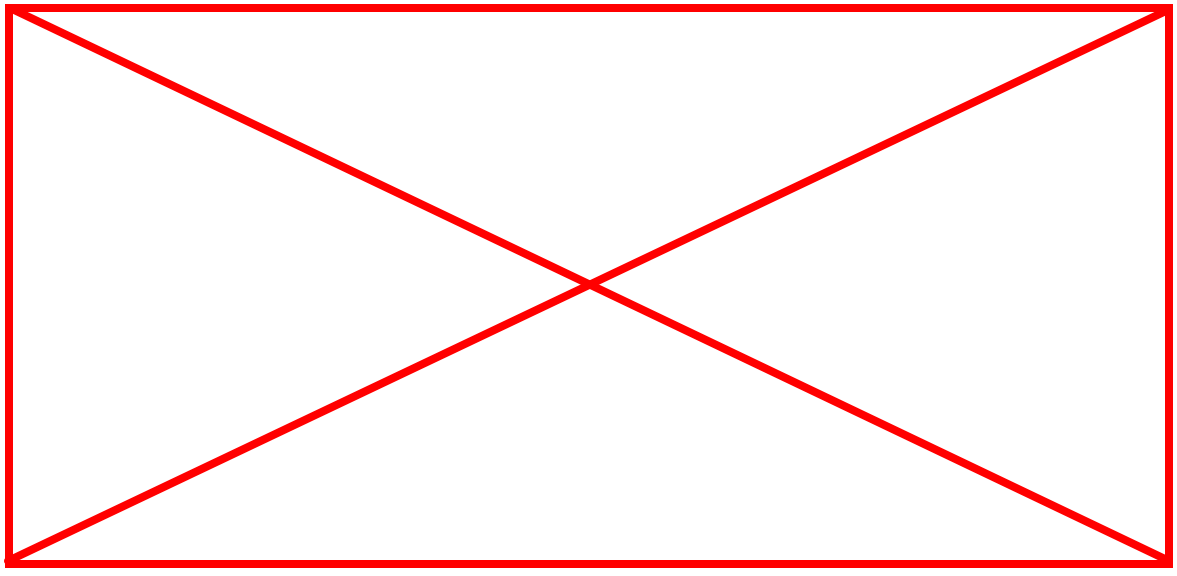
\includegraphics[width=\textwidth,height=240px,keepaspectratio]{pdf/noimage.png}
		\label{fig:esquematico_cbi}
		\indentedfont[15.2cm]{Elaboração própria (2021)}
	\end{figure}

	Alguns exemplos de equações:
	
	\[
		\binom{m+n}{m} = 
		\frac{(m+n)!}{m!n!} = 
		\frac{
			\overbrace{
				(m+n)(m+n-1)\cdots(n+1)
			}^{\clap{$m$ factors}}
		}{
			\underbrace{
				m(m-1)\cdots 1
			}_{\clap{$m$ factors}}}
	\]
	
	\begin{equation}
		\hat{x} = \hat{y} + a
	\end{equation}
	
	\begin{subequations}\label{eq-group1}
		\begin{align}
			\label{eq-lalala}
			\dot{x}
			&=	\begin{bmatrix}
				\dot{x_1} \\
				\dot{x_2} \\
				\dot{x_3} \\
			\end{bmatrix} 
			=	\begin{bmatrix}
				\dot{v_{C_1}} \\
				\dot{v_{C_2}} \\
				\dot{v_{C_3}} \\
			\end{bmatrix}
			=	\overbrace{
				\begin{bmatrix}
					0 & 559.44 & 0 \\
					-21.01 & -100.93 & 21.01 \\
					0 & 0 & -666.67
			\end{bmatrix}}^{A} x
			+	\overbrace{
				\begin{bmatrix}
					0 \\
					0 \\
					666.67
			\end{bmatrix}}^{B} u \\
			\label{eq-ssplanta_final}
			y
			&=	\overbrace{
				\begin{bmatrix}
					1 & 0 & 0 \\
			\end{bmatrix}}^{C} x
			+	\overbrace{
				\begin{bmatrix}
					0
			\end{bmatrix}}^{D} u
		\end{align}
	\end{subequations}
\chapter{Metodologia}
    
    É o caminho que se trilha, construindo, durante o percurso, os procedimentos e os instrumentos exigidos para se obter êxito no trabalho intelectual. É o momento da pesquisa em que se explicam, passo a passo, todos os procedimentos do estudo que permitiram que os resultados fossem atingidos, identificando os sujeitos com os quais foram coletados os dados, o modo como foram coletados, os instrumentos utilizados nessa coleta e a maneira como os dados foram analisados. 

    
\chapter{Métodos aplicados}

	Mostra-se como serão executados a pesquisa e o desenho metodológico que se pretende adotar: será do tipo quantitativa, qualitativa, descritiva, explicativa ou exploratória. Será um levantamento, um estudo de caso, uma pesquisa experimental, por exemplo. Segundo Gil 2006), a organização da metodologia depende do tipo de pesquisa a ser realizada. No entanto, alguns elementos devem ser apresentados, como:
	
	\begin{alineas}
	\item tipo de pesquisa: se é de natureza exploratória, descritiva ou explicativa.
	Convém, ainda, esclarecer acerca do tipo de delineamento a ser adotado pesquisa experimental, levantamento, estudo de caso, pesquisa bibliográfica);
	
	\item  população e amostra: envolve informações acerca do universo a ser estudado, da extensão da amostra e da maneira como será selecionada;
	\item coleta de dados: envolve a descrição das técnicas a serem utilizadas para a coleta de dados. Modelos de questionários ou testes deverão ser incluídos nessa parte. Se a pesquisa envolver técnicas de entrevista ou de observação, é também o momento de expor o assunto;
	\item análise dos dados: descrevem-se os procedimentos a serem adotados tanto
	para a análise quantitativa quanto qualitativa.
	\end{alineas}
\chapter{Resultados}
	Faz-se uma apresentação dos resultados a que se chegou a partir da pesquisa.
\chapter{Análise e Discussão}

	Faz-se uma exposição da análise obtida nos resultados da pesquisa, bem como uma discussão crítica a respeito deles.
\chapter{Considerações Finais}
    
    Nessa parte apresenta-se a síntese interpretativa dos principais argumentos usados, mostrando se os objetivos foram atingidos e se a(s) 31 hipótese(s) foi(foram) confirmada(s) ou rejeitada(s). Também se podem incluir recomendações e/ou sugestões para trabalhos futuros. Deve-se fazer uma rápida retomada dos capítulos que compõem o trabalho e uma espécie de autocrítica, fazendo um balanço a respeito dos resultados pela pesquisa.
    
    Atenção! A conclusão não constitui uma ideia nova ou um simples anexo sem importância ao trabalho. Pelo contrário, é nesse momento em que todas as ações do estudo são expostas, analisadas e finalizadas.
    
    Para melhor orientar-se, responda às seguintes questões:
    
    \begin{alineas}
	    \item a pesquisa resolve o problema, amplia a compreensão, mostra novas relações ou mesmo descobre outros problemas em relação ao originalmente escolhido?
	    \item a hipótese, ao final, foi confirmada ou refutada pela pesquisa?
	    \item os objetivos geral e específicos previamente definidos foram alcançados?
	    \item a metodologia de trabalho escolhida foi suficiente para a consecução de seus propósitos? houve necessidade, ao longo da pesquisa, de adotar outras técnicas ou procedimentos para lidar com situações não previstas?
	    \item a bibliografia previamente selecionada correspondeu às suas expectativas?
	\end{alineas}
    

% ----------------------------------------------------------
% ELEMENTOS PÓS-TEXTUAIS
% ----------------------------------------------------------
\postextual

% ----------------------------------------------------------
% Referências bibliográficas
% ----------------------------------------------------------
\bibliography{referencias}

% ----------------------------------------------------------
% Apêndices
% ----------------------------------------------------------
\begin{apendicesenv}
% Imprime uma página indicando o início dos apêndices
\partapendices

	\chapter{UM APÊNDICE}
	\label{ap:umalabel}
	
		Elemento opcional. "O(s) apêndice(s) são identificados por letras
		maiúsculas consecutivas, travessão e pelos respectivos títulos " (ASSOCIAÇÃO BRASILEIRA DE NORMAS TÉCNICAS, 2011). Os apêndices são textos e/ ou documentos elaborados pelo próprio autor para complementar o texto principal. Nos apêndices podem ser incluídos, por exemplo, questionários, modelos de entrevistas estruturadas ou transcrições de entrevistas utilizados
		no andamento da pesquisa.
		
		% Para incluir código, pesquisar sobre o pacote listingutf8
		% lstinputlisting{meucodigo.py}
	
\end{apendicesenv}

% ----------------------------------------------------------
% Anexos
% ----------------------------------------------------------
\begin{anexosenv}
% Imprime uma página indicando o início dos anexos
\partanexos

	\chapter{Um anexo}
	
	Elemento opcional. O anexo é um “texto ou documento não elaborado pelo autor, que serve de fundamentação, comprovação e ilustração” ASSOCIAÇÃO BRASILEIRA DE NORMAS TÉCNICAS, 2011). Também deve ser identificado por letras maiúsculas consecutivas, travessão e pelos respectivos títulos. No corpo do trabalho deve aparecer a indicação do anexo,
	sempre em ordem alfabética. 

\end{anexosenv}

%---------------------------------------------------------------------
% INDICE REMISSIVO
%---------------------------------------------------------------------
\phantompart
\printindex


\end{document}